
\documentclass[conference]{IEEEtran}
\usepackage{blindtext, graphicx}
\usepackage{url}
\usepackage{listings}
\usepackage{float}

\graphicspath{ {images/} }

% correct bad hyphenation here
\hyphenation{op-tical net-works semi-conduc-tor}


\begin{document}
%
% paper title
% can use linebreaks \\ within to get better formatting as desired
\title{Evaluation of the locality of the Mainline DHT}


% author names and affiliations
% use a multiple column layout for up to three different
% affiliations
\author{\IEEEauthorblockN{Marc Aymerich}
\IEEEauthorblockA{Universitat Politecnica de Catalunya}
Email: marc.aymerich@est.fib.upc.edu
\and
\IEEEauthorblockN{Unai Perez}
\IEEEauthorblockA{Universitat Politecnica de Catalunya}
Email: unai.perez@est.fib.upc.edu
\and
\IEEEauthorblockN{Be\~nat Txurruka}
\IEEEauthorblockA{Universitat Politecnica de Catalunya}
Email: benat.txurruka@est.fib.upc.edu}


% make the title area
\maketitle


\begin{abstract}
Community Networks (CN) are an emerging bottom-up model where communities of citizens build, operate and own open IP-based networks. In contrast to the traditional Internet, the core of these networks is build using unreliable wireless links and cheap low-end forwarding devices. For this reason, locality-aware applications become particular important in Community Networks.

Distributed Hash Tables (DHT) is a well known and mature decentralized key-value store system. Mainline DHT, the larger DHT deployed world-wide, is commonly used for storing BitTorrent peers, but it works for arbitrary data as well. Even though, Mainline DHT specifications do not provide mechanism that encourage locality, we have done so by choosing a particular \textit{Proximity Neighbour Selection} routing policy that encourages locality by choosing routing nodes with the lower round-trip-time (RTT).

In this paper we provide a preliminary study of the locality characteristics of the Mainline DHT using PYMDHT and one of its routing policies based on RTT measurements.
\end{abstract}


% Note that keywords are not normally used for peerreview papers.
\begin{IEEEkeywords}
DHT, MLDHT, API, P2P, CDNS, CN, RTT, ID, IP, UDP, TTL
\end{IEEEkeywords}

	

\section{Introduction}

Distributed Hash Table (DHT) is a decentralized system that provides look-up services similar to hash tables; (key, values) pairs are stored in a DHT, and any particular node can efficiently retrieve the associated value\cite{b30}. The decentralized nature and the scalability characteristics of DHT makes it the preferred way for storing shared state on P2P applications (e.g. peer lists). Kademlia and Mainline DHT are the most widely deployed DHTs world wide, creating overlay networks of millions of nodes \cite{b1}.

However, DHT not only serves good for storing peer swarms on P2P applications. DHT overlay networks are used on a large variety of Internet services. Some examples are, CDNS \cite{b2,b3}, application-level multicast, instant messaging, domain name services, web caching or distributed file systems.

On the other hand, DHT technologies are mainly evolving towards the Internet. And even though, emerging networks like Community Networks (CN)\footnote{\url{http://en.wikipedia.org/wiki/Community_network}} are based on the same fundamental technology than Internet, they also have their own discrepancies and peculiarities.

Community Networks raise from the dramatic drop of wireless network equipment cost over the last decade which has enabled end-users to build their own network independently from traditional telecommunications providers. This has a dramatic impact on the network properties. Most of its traffic flows through short-distance, low-throughput, high-latency wireless links, build with cheap low-end hardware.

The topology characteristics of Community Networks are also a bit different from the traditional Internet. On village-like environments, typical CN deployment may involve a single Access Point on the top-roof of the village from which all the clients connect to. On cities, usually the topology is a mesh-like network. Therefore, in both cases the network tends to forms clusters of nodes with a very few hops between each other but interconnected by long-distance inter-village wireless links.

Locality-aware applications become much important in CN because the cost of leaving the neighborhood is particularly expensive since it may involve transiting through several kilometers of unreliable microwave links, with significative packet loss, jitter, high latency and low throughput.

In this paper, we study the locality characteristics of DHT overlay on the context of Community Networks. In the next section background on DHT locality is presented.

%/////////////////////////////////////////////////////////////////////////////
\section{Background}

Network locality (proximity) in Distributed Hash Tables has been extensively studied \cite{b10, b11, b12, b31}. Three basic approaches have been suggested for exploring proximity in DHT protocols:

\subsection{Geographic Layout}

The node IDs are assigned in a manner that ensures that nodes that are close in the network topology are close in the node ID space. \textit{Geographic Layout} was explored as one technique to improve routing performance in CAN \cite{b4}. In one implementation, nodes measure the RTT between themselves and a set of landmark servers to compute the coordinates of the node in the CAN space.

\subsection{Proximity Routing}

The routing tables are built without taking network proximity into account but the routing algorithm chooses a nearby node at each hop from among the ones in the routing table. Proximity routing was first proposed in CAN \cite{b4}. It involves no changes to routing table construction and maintenance, because routing tables are built without taking network proximity into account.

\subsection{Proximity Neighbour Selection}

Routing table construction takes network proximity into account. Routing table entries are chosen to refer to nodes that are nearby in the network topology, among all live nodes with appropriate node IDs. Proximity neighbour selection is used in Tapestry and Pastry.

\textit{Geographic Layout} techniques are very effective for building overlays with a high degree of physical locality. However, we found that in the context of Community Networks it may not be the best choice. Network splits are common due to both, hardware malfunction (low-end hardware used) and human errors during management operations (intrinsic complexity of operating a highly decentralized network).

Because of network splits, a perfect locality based on \textit{Geographic Layout} may lead to entire portions of the DHT ID space inaccessible. In this sense, Proximity Routing and Proximity Neighbour Selection provides far better reliability since the Node IDs have nothing to do with the geographic location. 

Intuitively, \textit{Proximity Routing} may not work as good as \textit{Proximity Neighbour Selection}. Because the routing table is small (compared to the total number of nodes), there are not many candidates to choose from. Also prioritizing underlay locality over overlay locality may actually lead to an increase on the number of hops for DHT look-up operations.

We believe that \textit{Proximity Neighbour Selection} offers the best properties for deployment on CN. ID space is uniformly distributed over the whole network, making it robust, while good enough locality can still be achieved by choosing nearby nodes as routing table entries.

\section{Mainline DHT}

We based our DHT evaluation on Mainline DHT (MLDHT). MLDHT is a Kademlia-based Distributed Hash Table used by BitTorrent clients to find peers via the BitTorrent protocol. MLDHT is the largest DHT network currently deployed in the Internet, measures from 2013 show from 10 million to 25 million users, with a daily churn of at least 10 million [1].

Mainline DHT protocol is actually pretty simple, limited to four control messages:

\begin{enumerate}
\item \texttt{PING}: probe a node's availability. If the node fails to respond for some time, it will be purged out of the routing table
\item \texttt{FIND\_NODE}: given a target ID, this message is used to find the \{k\} closest neighbors of the ID
\item \texttt{GET\_PEERS}: given an infohash, get the initial peer set. Notice that BitTorrent peer locality is also an interesting factor, but its evaluation is not the objective of this work
\item \texttt{ANNOUNCE\_PEER}: a peer announces it belongs to a swarm
\end{enumerate}

Its simplicity and the fact that it is a widely deployed protocol makes its evaluation study somehow easier, since the complexity is low and there are several MLDHT implementations to choose from. We looked at libtorrent and PYMDHT.

libtorrent \cite{b6} was our first consideration, is a well known open source implementation of BitTorrent protocol and it has support for Mainline DHT. However, we quickly found out that its public API provides little information about the DHT routing state, only providing the node ID of each entry, not the IP address nor RTT measurements. This is not surprising since its design is focused on BitTorrent applications, not on DHT routing evaluation. Also libtorrent implements a highly tune and complicated routing algorithm with a lot of corner cases and optimizations making its behaviour less predictable \cite{b1}.

PYMDHT \cite{b8} is a flexible Python implementation of the Mainline DHT protocol, specifically designed for MDHT evaluation. This is the main reason why we choose PYMDHT over libtorrent, even though PYMDHT current state is experimental, the codebase has room for improvement and there is no public documentation available.

Mainline DHT, as described in BitTorrent Enhancement Proposal 5 (BEP5) \cite{b9}, does not consider any means for locality. However, implementers of this DHT are free to choose whatever routing policy they wish to. In the case of PYMDHT a plugging system is in place for easily switching between routing policies. Moreover, the library ships with an implementation of a \textit{Proximity Neighbour Selection} routing policy defined by NICE \cite{b18}, based on RTT measurements, which is very convenient as a foundation for our locality evaluation.

\section{MLDHT Locality Evaluation on \\ Community Lab}

The testbed of choice for our evaluation is Community Lab\footnote{\url{http://community-lab.net/}}, a Community Networks Testbed by the CONFINE project that provides a global facility for experimentation with network technologies and services for Community Networks \cite{b16}.

Our experiments take place on a 140 node slice, the whole set of Community Lab nodes at this time. Unfortunately, the amount of effectively available nodes is severely reduced by several factors.
\begin{itemize}
\item Around 63 nodes are in offline state most of the time
\item 20 nodes do not have Internet connectivity, needed for installing
dependencies
\item 5 nodes report a "Fail allocate" state
\item 3 nodes remian in "Unknown" state
\item From those online, 17 do not have IP connectivity with the rest \footnote{\url{https://github.com/glic3rinu/MLDHT-locality/blob/master/results/hops}}. Some of them because a lack of public IP addresses and others because of inadequate federation between CN
\end{itemize}

This leaves us with a total amount of around 26 usable nodes. Moreover, we have seen PYMDHT instances to randomly crash in several occasions, further decreasing the total number of operative DHT nodes.

Because of the reduced number of available nodes in our testbed, special care is needed in order to design experiments that produce any significant result about the locality properties. Remember that MLDHT is build with Internet scale in mind, with millions of nodes in size. The original Mainline DHT as defined in BEP5 specifies an ID space of 160 bits, which translates to 160 buckets, a lot more than nodes on our testbed.

Some changes on the original PYMDHT implementation had been performed in order to accommodate our tiny DHT.
\begin{itemize}
\item \texttt{DEFAULT\_NUM\_NODES}, 8 by default, controls the number of nodes per bucket and it has been reduced to 1 in order to have a larger set of competing nodes for each bucket
\item \texttt{MAX\_NUM\_TIMEOUTS}, 2 by default, determines how many sequential timeouts are allowed for a routing entry before being replaced. We set its value to -1 in order to have a faster convergence of routing table entries locality
\item  The original NICE RTT routing policy applies a decreasing factor to the candidate RTT

\begin{lstlisting}[language=python]
rnode.rtt * (1 - (rnode_age / 7200))
\end{lstlisting}

For instance, when routing node has been in the bucket for 30 minutes, a candidate's RTT must be at most 25\% of the routing node's RTT (ie. two times faster). After two hours, a routing node cannot be replaced by this method. In order to give RTT a higher weight, this factor has been eliminated from the conditions needed for new routing entries.
\item  Reducing the ID space, and thus reducing the number of buckets, has been proposed but finally not implemented because multiple parts of PYMDHT's codebase makes assumptions about the ID space size. However, we use crafted node IDs and infohashes (not randomly generated), in order to artificially reduce the effective amount of buckets (e.g. generate some IDs that belong to a particular bucket).
\end{itemize}

Considering that, round-trip time (RTT) is the only locality-related metric used by our routing policy, one may argue that RTT may not be reliable enough in CN because of the high jitter of most wireless links (latency variation). In that effect, distance measured by UDP packets with a crafted time-to-live (TTL), a.k.a. traceroute, may also be an interesting metric to consider for inclusion on the DHT routing algorithm. However, this metric is not available at this time.

By executing traceroute on each node\footnote{\url{https://github.com/glic3rinu/MLDHT-locality/blob/master/traceroute.sh}} we have calculated the average number of hops on the whole network. Which in our case is 7.5 (with an standard deviation of 5.2). This number can be used as a reference point in order to evaluate how good or bad is the locality in our nodes routing tables.

Additionally, we have to take into account that some nodes are between 11 and 18 hops from the nearest node. We have considered to threat those nodes as outliers, but we finally discarded this idea since doing so will reduce even further the amount of nodes on our DHT. And because of the topology characteristics of Community Lab, almost all remaining nodes will be sitting on a laboratory, one next to the other.

In the next sections the results of locality evaluation of the DHT routing table entries are presented. Notice that, because of the limited size of our DHT, the workload of each experiment has been crafted in order to artificially promote locality rather than focus on more realistic workloads. All the experiments and results are publicly available at Github\footnote{\url{https://github.com/glic3rinu/MLDHT-locality}}.


\subsection{High Load Workload}

Each DHT node announces N infohashes and periodically performs a \texttt{GET\_PEERS} of all the other nodes announced infohashes, after randomly waiting between 60 and 300 seconds. The total number of \texttt{GET\_PEERS} queries performed on the DHT every minute will be greater than $\frac{1}{4} (NUM\_NODES-1) \cdot N$, since an initial query may involve several recursive queries before completion.

\begin{figure}
    \includegraphics[width=\columnwidth]{exp1,1-ids1-cache0.png}
    \caption{\textit{High Load Workload} results. Sub-figure 1: average number of hops on the routing table. Sub-figure 2: average latency per node on the the routing table. Sub-figure 3: green triangles is the average of the average number of hops, blue squares is the average of the average latency.}
    \label{fig:exp1,1-ids1-cache0}
\end{figure}

Figure \ref{fig:exp1,1-ids1-cache0} shows an steady average of 6 hops, a value very close to the network mean 7.5. This is because nodes perform queries to random buckets, and because we have an average of less than one node per bucket $26/160$, there is little chance for the routing policy to perform selection based on RTT measurements, only the farthest buckets from each node ID has several competing routing nodes.

A second round of this workload has been executed but now with caching enabled. After a very few rounds \texttt{GET\_PEERS} results are cached over several nodes. Thus, giving more chance to lower latency nodes to be selected as routing nodes.

\begin{figure}
    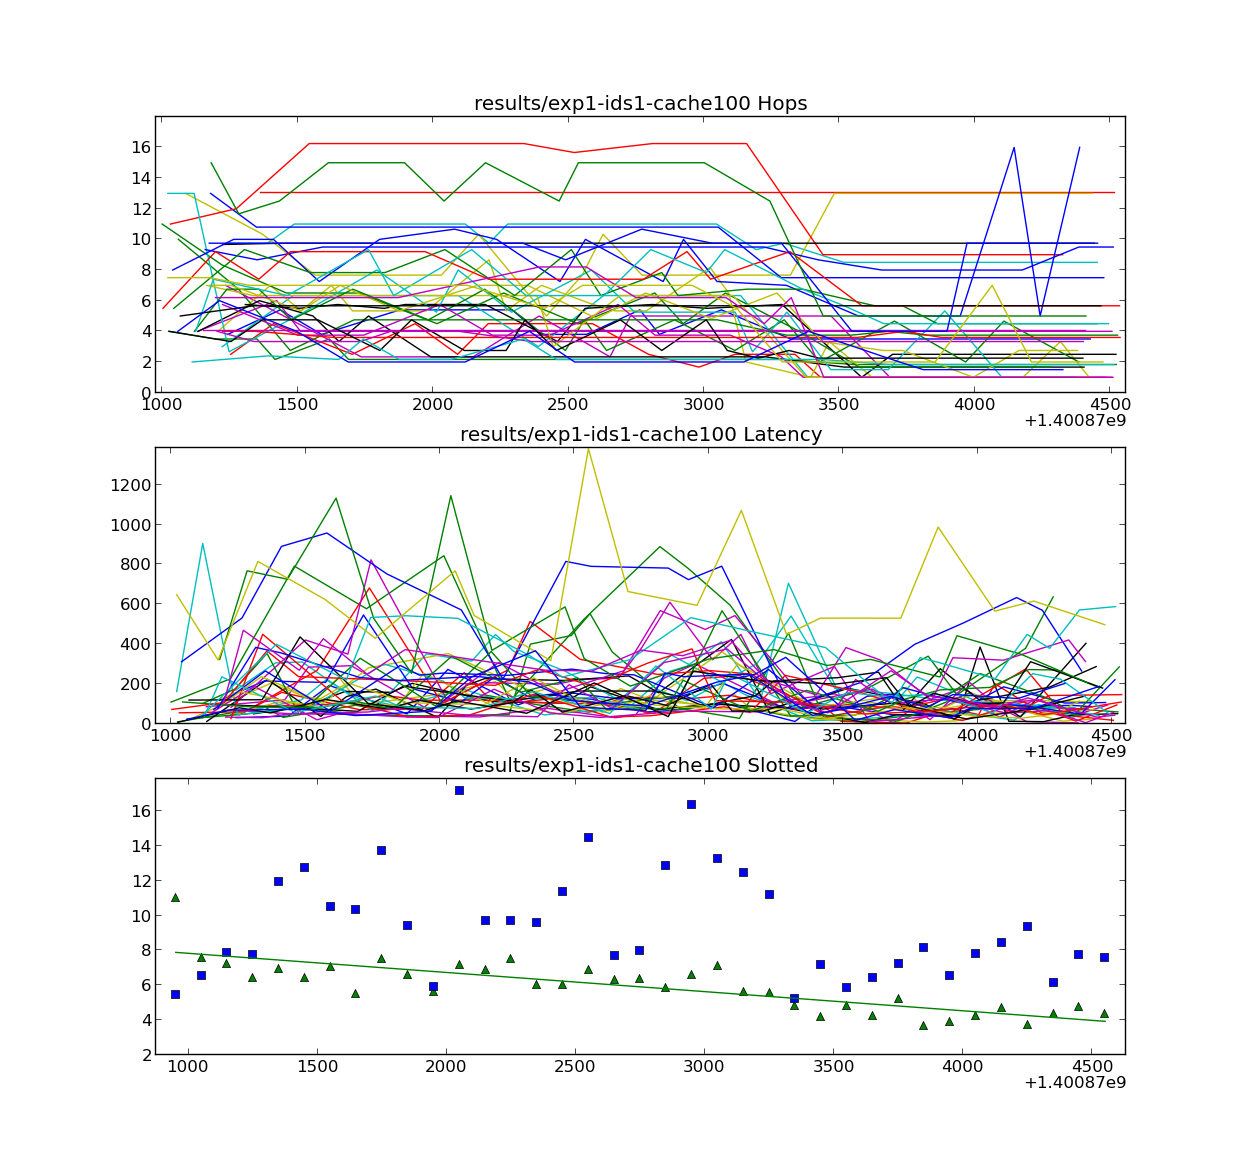
\includegraphics[width=\columnwidth]{exp1-ids1-cache100.png}
    \caption{\textit{High Load Workload with caching} results. Sub-figure 1: average number of hops on the routing table. Sub-figure 2: average latency per node on the the routing table. Sub-figure 3: green triangles is the average of the average number of hops, blue squares is the average of the average latency.}
    \label{fig:exp1-ids1-cache100}
\end{figure}

In figure \ref{fig:exp1-ids1-cache100} we see how caching seems to makes convergence to a better locality value, but repetitions of this same experiments show mixed results. At this point we are not able to conclude that caching leads to better locality, at least in our 26 node DHT. However, caching seems to affect the patter on the routing table hops and latencies, compared with fig. \ref{fig:exp1,1-ids1-cache0}.

In order to see how churn affects locality we have divided the experiment in 3 phases. In each phase 1/3 of our nodes are added to the DHT. The idea behind this is to gradually increase the number of nearby nodes and see how the routing algorithm adapts to it.

\begin{figure}
    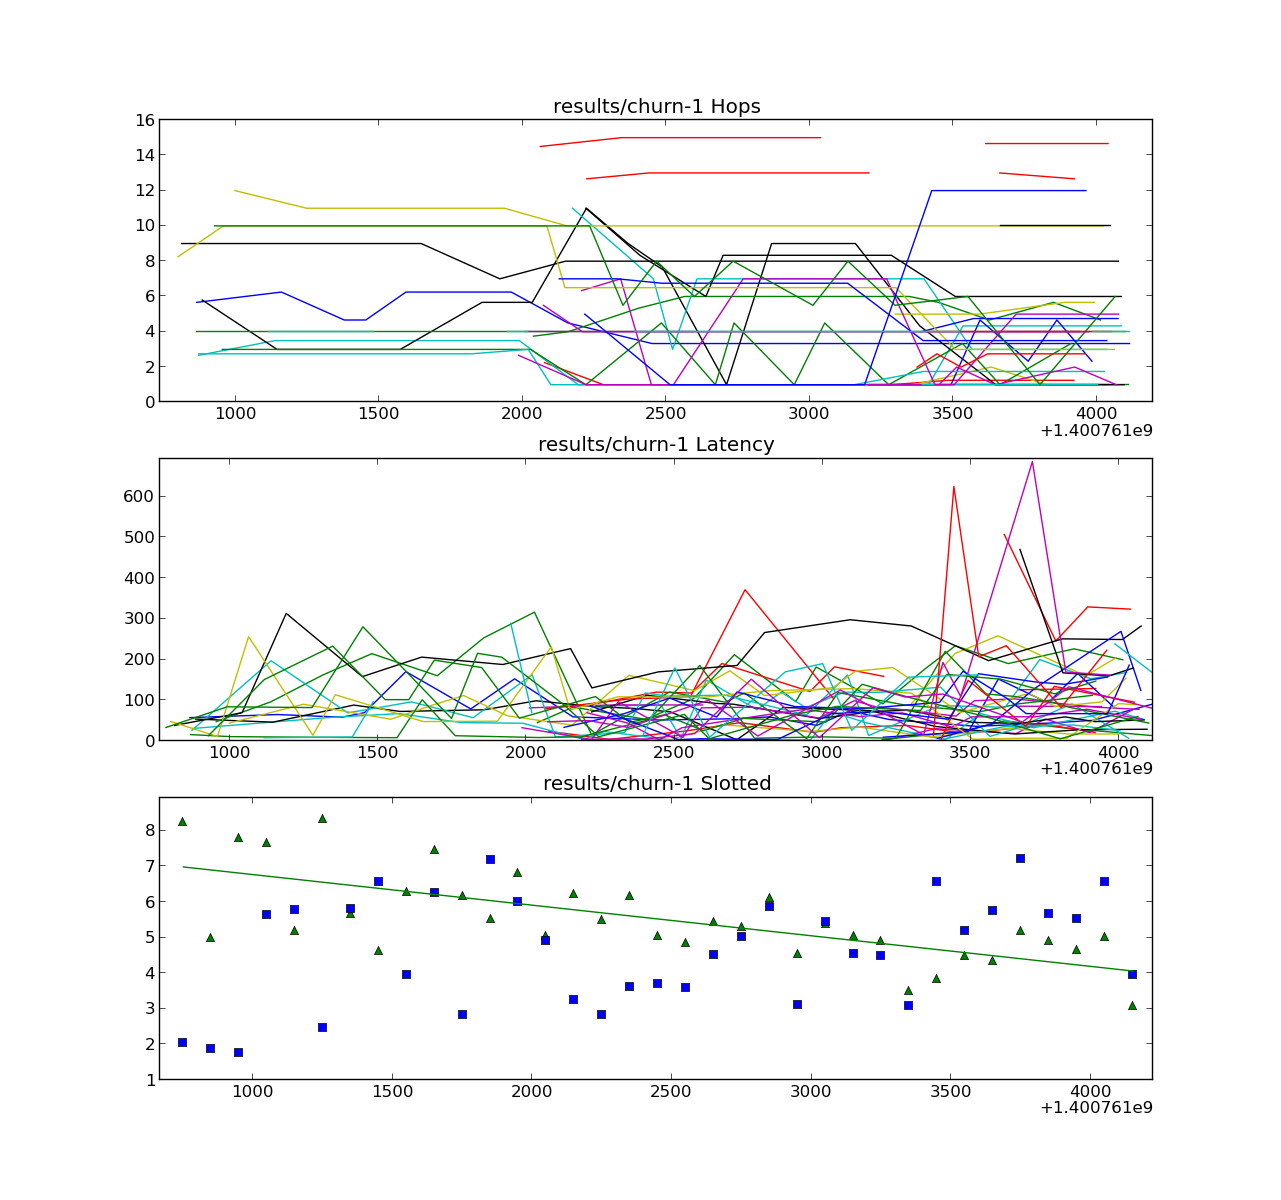
\includegraphics[width=\columnwidth]{churn-1.png}
    \caption{\textit{High Load Workload with churn} results. Sub-figure 1: average number of hops on the routing table. Sub-figure 2: average latency per node on the the routing table. Sub-figure 3: green triangles is the average of the average number of hops, blue squares is the average of the average latency.}
    \label{fig:churn-1}
\end{figure}

In Figure \ref{fig:churn-1} we can see the gradual selection of nearer nodes as they become available during the 3 phases of the experiment.

\subsection{Close IDs Workload}

All node's ID 120 most significant bits are the same, also an infohash with the same characteristics is inserted in the DHT and all the nodes perform periodic \texttt{GET\_PEERS} requests of this infohash.

This workload is designed to characterize the locality of nearby nodes in terms of the overlay network. Since our DHT size is very small, we decided to force all the nodes to be compacted on the same portion of the ID space in order to determine how the routing policy performs with some logical nearby nodes.

\begin{figure}
    \includegraphics[width=\columnwidth]{exp3,2-cache100-2-original.png}
    \caption{\textit{Close IDs Workload} results. Sub-figure 1: average number of hops on the routing table. Sub-figure 2: average latency per node on the the routing table. Sub-figure 3: green triangles is the average of the average number of hops, blue squares is the average of the average latency.}
    \label{fig:exp3,2-cache100-2-original}
\end{figure}

Because of the bucket distribution, based on logarithmic distance, much more buckets are reserved for nearby IDs. Figure \ref{fig:exp3,2-cache100-2-original} shows an steady average of 4 hops, better than the average number of hops on the whole network (7.5). Our guess is that the routing algorithm stabilizes very quickly during bootstrap and then the routing table remains intact because of the lack of churn. A sign of this early stabilization is the flat patter on the number of hops and latencies plots.

\begin{figure}
    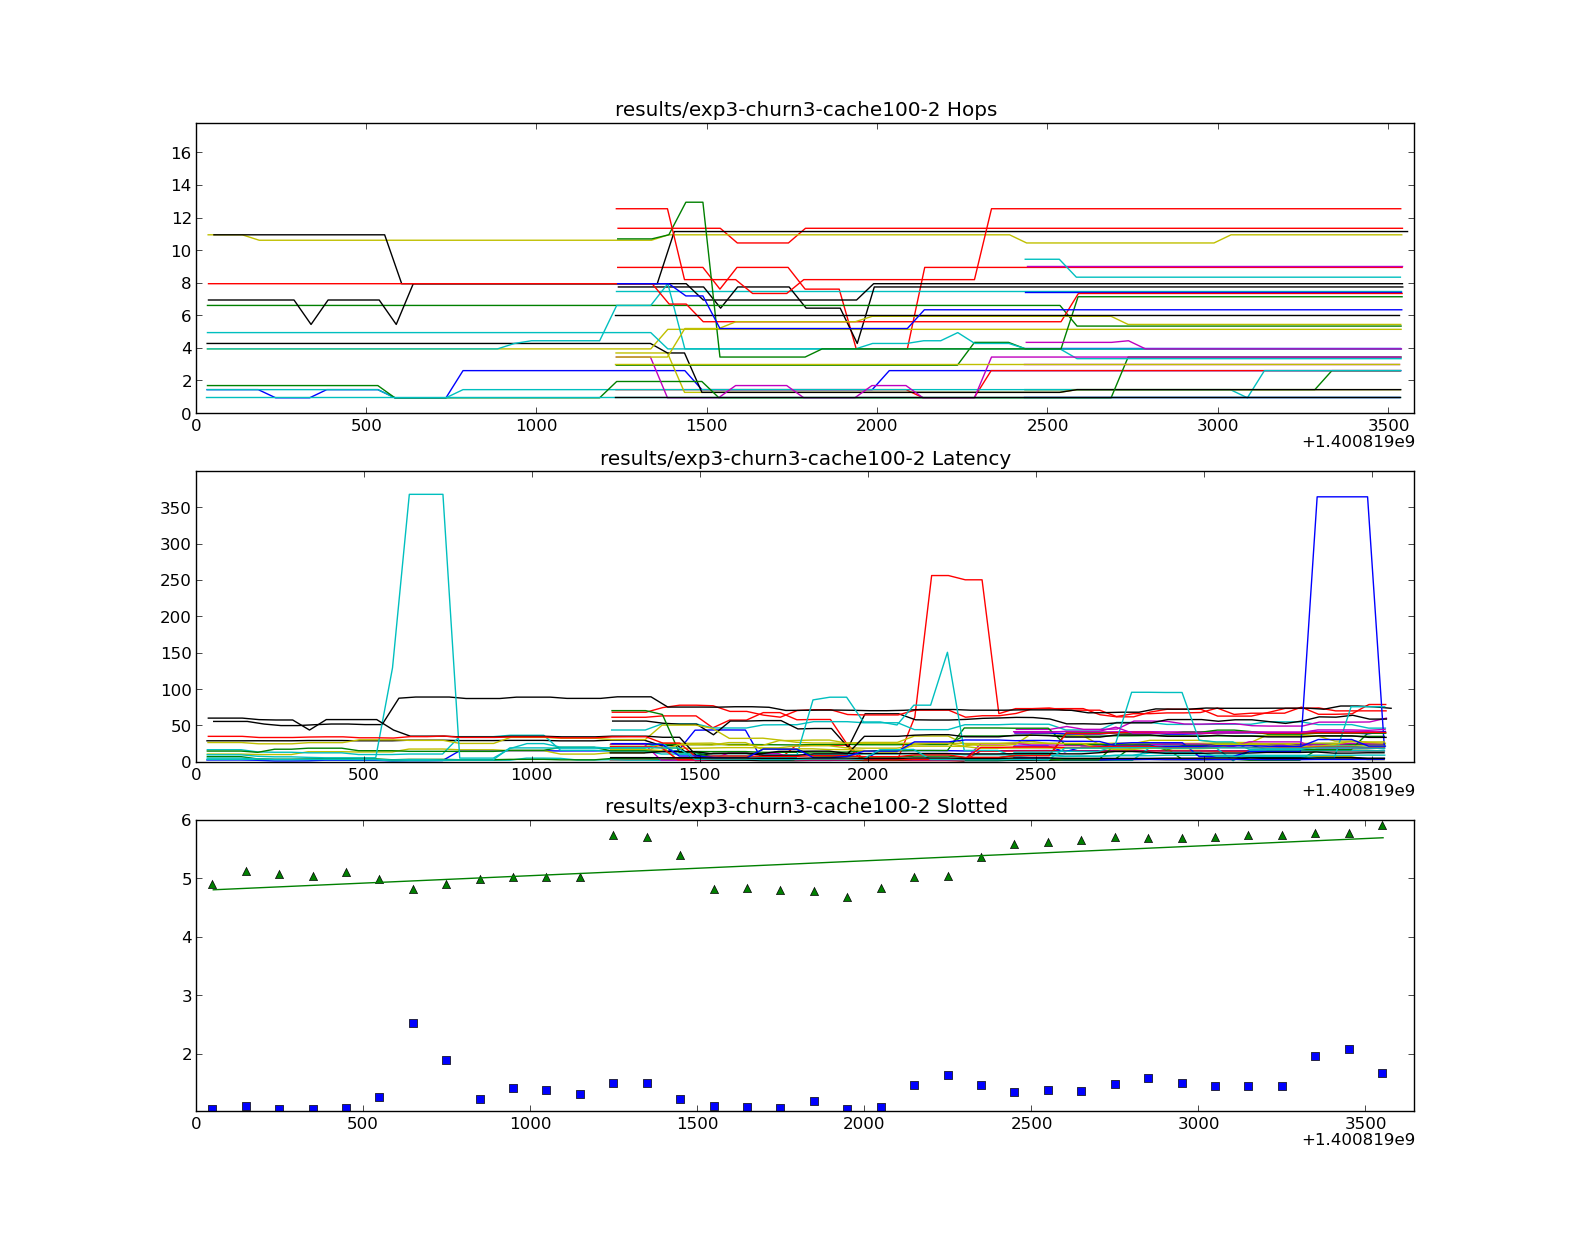
\includegraphics[width=\columnwidth]{exp3-churn3-cache100-2.png}
    \caption{\textit{Close IDs Workload with churn} results. Sub-figure 1: average number of hops on the routing table. Sub-figure 2: average latency per node on the the routing table. Sub-figure 3: green triangles is the average of the average number of hops, blue squares is the average of the average latency.}
    \label{fig:exp3-churn3-cache100-2}
\end{figure}

In Figure \ref{fig:exp3-churn3-cache100-2} we see that churn actually harms locality. The reason might be that 26 nodes are not enough to fill the amount of buckets assigned for closer IDs (logarithmic distribution), and thus, close ID nodes are preferred over the physically near ones.


\subsection{Lonely Node Workload}

This experiment also uses crafted node IDs to force all node's ID being in the same bucket from the lonely node point of view. We want to create a lot of bucket competition on the lonely node routing table and validate that the physically nearest node is always chosen.

Interestingly enough, Community Lab topology includes the type of node clustering commonly seen in Community Network villages and described on the introductory chapter. In the case of Community Lab those are the nodes at UPC-Lab, where only one forwarding device sits between the nodes \cite{b19}.

The lonely node is selected from this cluster since it have plenty of nearby candidates to choose from. Figure \ref{fig:exp2,2-cache100-node39-original} illustrates the results of this experiment.

\begin{figure}
    \includegraphics[width=\columnwidth]{exp2,2-cache100-node39-original.png}
    \caption{\textit{Lonely Node Workload} results. Sub-figure 1: average number of hops on the routing table. Sub-figure 2: average latency per node on the the routing table. Sub-figure 3: green triangles is the average of the average number of hops, blue squares is the average of the average latency.}
    \label{fig:exp2,2-cache100-node39-original}
\end{figure}


\subsection{Two Buckets Workload}

Perhaps this experiment is the most interesting of all. In order to effectively reduce the number of buckets on the overlay we have generated node IDs that belong to two different buckets. And then each group of nodes perform \texttt{GET\_PEERS} queries to the other group's infohash. Therefore, we have plenty of routing nodes competing for the same position on the routing tables. We call this bucket, the \textit{competing bucket}.

\begin{figure}
    \includegraphics[width=\columnwidth]{exp4,2-cache100-nodes1.png}
    \caption{\textit{Two Buckets Workload} results. Sub-figure 1: average number of hops per node on the \textit{competing bucket}. Sub-figure 2: average latency per node on the \textit{competing bucket}. Sub-figure 3: green triangles is the average of the average number of hops, blue squares is the average of the average latency.}
    \label{fig:exp4,2-cache100-nodes1}
\end{figure}

Figure \ref{fig:exp4,2-cache100-nodes1} shows the results, in this case we only measure the \textit{competing bucket} and not the buckets that belong to the node's own group. The results are not as good as expected, 5 hops on average, below the average hops on the network (7.5). Perhaps the fact that some nodes have the nearest neighbor at 11-18 hops makes the average number of hops a bad locality evaluator. Maybe a more powerful statistical analysis of the results could provide a partial, or total, explanation to this bad score. Additionally, Figure \ref{fig:exp4,2-cache100-nodes1} shows that MLDHT needs some minutes to stabilize the routing table. 

\section{Future Work}

The main limitation of our evaluation is the reduced number of nodes in our testbed. Further analysis should be performed in order to better understand the locality characteristics of Mainline DHT, specially under realistic workloads.

Solely using the average number of hops may not be a good enough locality evaluator. A better one could be the average number of hops of the routing entries over the average number of hops to other nodes, ($\frac{avg(routing\_hops)}{avg(total\_hops}$). Or even better, the potential optimal value over the current value. In short, making the values dependent of each node vision of the network will give a better fit.

Measurements of the number of underlay hops of the \texttt{ANNOUNCE\_PEER} and \texttt{GET\_PEERS} queries are missing in our evaluation, but are key measurements to better understand locality in a DHT.

An interesting extension of our work could be estimate how locality-aware routing policy affects response time and other performance characteristics of Mainline DHT.


% needed in second column of first page if using \IEEEpubid
%\IEEEpubidadjcol

% An example of a floating figure using the graphicx package.
% Note that \label must occur AFTER (or within) \caption.
% For figures, \caption should occur after the \includegraphics.
% Note that IEEEtran v1.7 and later has special internal code that
% is designed to preserve the operation of \label within \caption
% even when the captionsoff option is in effect. However, because
% of issues like this, it may be the safest practice to put all your
% \label just after \caption rather than within \caption{}.
%
% Reminder: the "draftcls" or "draftclsnofoot", not "draft", class
% option should be used if it is desired that the figures are to be
% displayed while in draft mode.
%
%\begin{figure}[!t]
%\centering
%\includegraphics[width=2.5in]{myfigure}
% where an .eps filename suffix will be assumed under latex, 
% and a .pdf suffix will be assumed for pdflatex; or what has been declared
% via \DeclareGraphicsExtensions.
%\caption{Simulation Results}
%\label{fig_sim}
%\end{figure}

% Note that IEEE typically puts floats only at the top, even when this
% results in a large percentage of a column being occupied by floats.


% An example of a double column floating figure using two subfigures.
% (The subfig.sty package must be loaded for this to work.)
% The subfigure \label commands are set within each subfloat command, the
% \label for the overall figure must come after \caption.
% \hfil must be used as a separator to get equal spacing.
% The subfigure.sty package works much the same way, except \subfigure is
% used instead of \subfloat.
%
%\begin{figure*}[!t]
%\centerline{\subfloat[Case I]\includegraphics[width=2.5in]{subfigcase1}%
%\label{fig_first_case}}
%\hfil
%\subfloat[Case II]{\includegraphics[width=2.5in]{subfigcase2}%
%\label{fig_second_case}}}
%\caption{Simulation results}
%\label{fig_sim}
%\end{figure*}
%
% Note that often IEEE papers with subfigures do not employ subfigure
% captions (using the optional argument to \subfloat), but instead will
% reference/describe all of them (a), (b), etc., within the main caption.


% An example of a floating table. Note that, for IEEE style tables, the 
% \caption command should come BEFORE the table. Table text will default to
% \footnotesize as IEEE normally uses this smaller font for tables.
% The \label must come after \caption as always.
%
%\begin{table}[!t]
%% increase table row spacing, adjust to taste
%\renewcommand{\arraystretch}{1.3}
% if using array.sty, it might be a good idea to tweak the value of
% \extrarowheight as needed to properly center the text within the cells
%\caption{An Example of a Table}
%\label{table_example}
%\centering
%% Some packages, such as MDW tools, offer better commands for making tables
%% than the plain LaTeX2e tabular which is used here.
%\begin{tabular}{|c||c|}
%\hline
%One & Two\\
%\hline
%Three & Four\\
%\hline
%\end{tabular}
%\end{table}


% Note that IEEE does not put floats in the very first column - or typically
% anywhere on the first page for that matter. Also, in-text middle ("here")
% positioning is not used. Most IEEE journals use top floats exclusively.
% Note that, LaTeX2e, unlike IEEE journals, places footnotes above bottom
% floats. This can be corrected via the \fnbelowfloat command of the
% stfloats package.



\section{Conclusion}
In this paper we have shown that locality in Mainline DHT can be achieved with a very simple routing policy bases on \textit{Proximity Neighbour Selection} with RTT measurements. We also show that Mainline DHT, as defined in BEP5, is designed specifically for Internet scale deployments, changes on the DHT dimensions are required in order to properly accommodate smaller deployments, for instance, thus on Community Networks.

We have also seen the limitations of having an small number of nodes. Leading to the need of crafting node IDs and infohashes and to design experiments very carefully in order to have any significant result.

We consider this study very preliminary, further evaluations, with more powerful statistical analysis and more nodes, are needed in order to better quantify the locality properties and their performance implications.

% use section* for acknowledgement
\section*{Acknowledgment}

%The authors would like to thank...

We would like to thank Raul Jimenez from Royal Institute of Technology (KTH) and
Leandro Navarro from Universitat Politecnica de Catalunya (UPC), for their advice, help and interest during the realization of this project.


% Can use something like this to put references on a page
% by themselves when using endfloat and the captionsoff option.
\ifCLASSOPTIONcaptionsoff
  \newpage
\fi



% trigger a \newpage just before the given reference
% number - used to balance the columns on the last page
% adjust value as needed - may need to be readjusted if
% the document is modified later
%\IEEEtriggeratref{8}
% The "triggered" command can be changed if desired:
%\IEEEtriggercmd{\enlargethispage{-5in}}

% references section

% can use a bibliography generated by BibTeX as a .bbl file
% BibTeX documentation can be easily obtained at:
% http://www.ctan.org/tex-archive/biblio/bibtex/contrib/doc/
% The IEEEtran BibTeX style support page is at:
% http://www.michaelshell.org/tex/ieeetran/bibtex/
%\bibliographystyle{IEEEtran}
% argument is your BibTeX string definitions and bibliography database(s)
%\bibliography{IEEEabrv,../bib/paper}
%
% <OR> manually copy in the resultant .bbl file
% set second argument of \begin to the number of references
% (used to reserve space for the reference number labels box)
\begin{thebibliography}{1}

%\bibitem{IEEEhowto:kopka}
%H.~Kopka and P.~W. Daly, \emph{A Guide to \LaTeX}, 3rd~ed.\hskip 1em plus
%  0.5em minus 0.4em\relax Harlow, England: Addison-Wesley, 1999.

\bibitem{b1}
Wang, Liang, and Jussi Kangasharju. "Measuring large-scale distributed systems: case of BitTorrent Mainline DHT." Peer-to-Peer Computing (P2P), 2013 IEEE Thirteenth International Conference on. IEEE, 2013.

\bibitem{b2}
Akamai, \url{www.akamai.com}

\bibitem{b3}
Digital island, \url{http://www.digitalisland.co.nz/}

\bibitem{b4}
Exploring Network Proximity

\bibitem{b5}
LDHT

\bibitem{b6}
Rasterbar Software, \emph{libtorrent}, \url{http://www.rasterbar.com/products/libtorrent/}, 2005

\bibitem{b8}
Raul Jimenez, \emph{pymdht}, \url{https://github.com/rauljim/pymdht}, 2009-2012

\bibitem{b9}
BitTorrent Enhancement Proposals, \url{http://www.bittorrent.org/beps/bep_0005.html}

\bibitem{b10}
Wu, Weiyu, et al. "LDHT: locality-aware distributed hash tables." Information Networking, 2008. ICOIN 2008. International Conference on. IEEE, 2008.

\bibitem{b11}
Ferreira, Ronaldo A., Suresh Jagannathan, and Ananth Grama. "Locality in structured peer-to-peer networks." Journal of Parallel and Distributed Computing 66.2 (2006): 257-273.

\bibitem{b12}
Zhou, Shuheng, Gregory R. Ganger, and Peter Alfons Steenkiste. "Location-based node ids: Enabling explicit locality in dhts." (2003).

\bibitem{b16}
CONFINE Project, \url{http://confine-project.eu/}

\bibitem{b18}
UMD, \url{http://www.cs.umd.edu/projects/nice/}

\bibitem{b19}
Community-Lab, \url{http://monitor.confine-project.eu:8000/networktrace/}

\bibitem{b30}
Wikipedia, \url{http://en.wikipedia.org/wiki/Distributed_hash_table}

\bibitem{b31}
Castro, Miguel, et al. "Exploiting network proximity in distributed hash tables." International Workshop on Future Directions in Distributed Computing (FuDiCo). 2002.

\end{thebibliography}

% biography section
% 
% If you have an EPS/PDF photo (graphicx package needed) extra braces are
% needed around the contents of the optional argument to biography to prevent
% the LaTeX parser from getting confused when it sees the complicated
% \includegraphics command within an optional argument. (You could create
% your own custom macro containing the \includegraphics command to make things
% simpler here.)
%\begin{biography}[{\includegraphics[width=1in,height=1.25in,clip,keepaspectratio]{mshell}}]{Michael Shell}
% or if you just want to reserve a space for a photo:

\begin{IEEEbiography}[{\includegraphics[width=1in,height=1.25in,clip,keepaspectratio]{picture}}]{John Doe}
\blindtext
\end{IEEEbiography}

% You can push biographies down or up by placing
% a \vfill before or after them. The appropriate
% use of \vfill depends on what kind of text is
% on the last page and whether or not the columns
% are being equalized.

%\vfill

% Can be used to pull up biographies so that the bottom of the last one
% is flush with the other column.
%\enlargethispage{-5in}




% that's all folks
\end{document}



